\documentclass[11pt]{article}
\usepackage[a4paper,margin=21mm]{geometry}
\usepackage{amsmath,amssymb,booktabs,array}
\usepackage{tikz}
\usepackage[T1]{fontenc}
\usepackage{lmodern}
\usepackage[hidelinks]{hyperref}
\usepackage{listings}
\lstset{basicstyle=\ttfamily\small,breaklines=true,columns=fullflexible,frame=single}
\setlength{\parindent}{0pt}
\setlength{\parskip}{6pt}
\setlength{\emergencystretch}{1.5em}
\newcommand{\mos}[4]{\begin{scope}[shift={(#1,#2)}]
\draw (0,.24)--(0,-.24);
\draw (0,.20)--(.25,.20)--(.25,.5);
\draw (0,-.20)--(.25,-.20)--(.25,-.5);
\draw (-.16,.23)--(-.16,-.23);
\ifnum#4=1\draw (-.26,0) circle (.06);\draw (-.75,0)--(-.32,0);\else\draw (-.75,0)--(-.16,0);\fi
\node[anchor=east,font=\small] at (-.76,0) {$#3$};
\end{scope}}
\newcommand{\ground}[2]{\draw (#1,#2)--(#1,{#2-.12});\draw ({#1-.17},{#2-.12})--({#1+.17},{#2-.12});\draw ({#1-.11},{#2-.20})--({#1+.11},{#2-.20});}
\newcommand{\rail}[3]{\draw (#1,#2)--(#1,{#2+.15});\node[above,font=\small] at (#1,{#2+.15}) {$#3$};}
\newcommand{\outputnode}[3]{\fill (#1,#2) circle (.04);\draw (#1,#2)--({#1+.7},#2) node[right] {$#3$};}
\begin{document}
\begin{center}{\Large\bfseries Introduction to VLSI Design, 2015}\par{\large Homework 4: mirror and domino full adders}\end{center}
\section*{Functions, technology, and numerical target}
For inputs A, B, C, the carry is $C_o=AB+AC+BC$ and sum is $S=(A+B+C)\bar C_o+ABC=A\oplus B\oplus C$. Both original parts are completed at schematic SPICE level using CIC018 TT $N\_18/P\_18$, $V_{DD}=1.8$ V, and 25 C. No layout is requested in this homework or represented as completed.

The phrase $t_r=t_f$ needs an electrical convention. All input and clock ramps have equal 20 ps rise/fall times. Device sizing additionally balances each external output's \emph{worst} 10--90\% rise time and 90--10\% fall time to within 3\%, over all covered cases, with 1 fF external load per output and declared 0.18 $\mu$m diffusion extensions. Exact equality for every distinct path or every corner cannot follow from one fixed sizing. Final verification uses a 0.2 ps maximum solver step.

\section*{(a) 28-transistor mirror adder}
Use a 10T self-dual carry-complement core followed by a 2T inverter. The sum-complement core has 7 PMOS and 7 NMOS devices, followed by another 2T inverter. Total: $10+2+14+2=28$ MOSFETs. NMOS bodies use VSS; PMOS bodies use VDD. The carry PDN computes $C(A+B)+AB$; its mirror PUN conducts for $\bar C(\bar A+\bar B)+\bar A\bar B$. The sum PDN computes $\bar C_o(A+B+C)+ABC$; its mirror PUN is the complementary network under the internally generated carry relation.

\begin{center}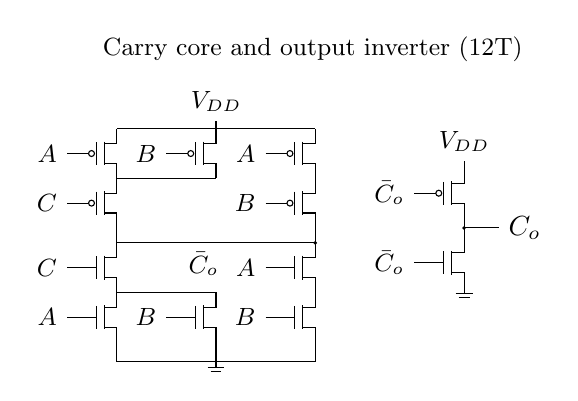
\begin{tikzpicture}[scale=.63]
% mirror carry PUN
\mos{0}{5.5}{A}{1}\mos{2}{5.5}{B}{1}\mos{0}{4.5}{C}{1}\mos{4}{5.5}{A}{1}\mos{4}{4.5}{B}{1}
\draw (.25,6)--(4.25,6);\rail{2.25}{6}{V_{DD}}\draw (.25,5)--(2.25,5);\draw (.25,4)--(.25,3.7)--(4.25,3.7)--(4.25,4);\fill (4.25,3.7) circle (.04);\node[below,font=\small] at (2,3.7){$\bar C_o$};
% mirror carry PDN
\mos{0}{3.2}{C}{0}\mos{0}{2.2}{A}{0}\mos{2}{2.2}{B}{0}\mos{4}{3.2}{A}{0}\mos{4}{2.2}{B}{0}
\draw (.25,2.7)--(2.25,2.7);\draw (.25,1.7)--(.25,1.3)--(4.25,1.3)--(4.25,1.7);\draw (2.25,1.7)--(2.25,1.3);\ground{2.25}{1.3}
\mos{7}{4.7}{\bar C_o}{1}\mos{7}{3.3}{\bar C_o}{0}\rail{7.25}{5.2}{V_{DD}}\ground{7.25}{2.8}\draw (7.25,3.8)--(7.25,4.2);\outputnode{7.25}{4}{C_o}
\node[font=\small] at (4.2,7.6){Carry core and output inverter (12T)};
\end{tikzpicture}\end{center}
\begin{center}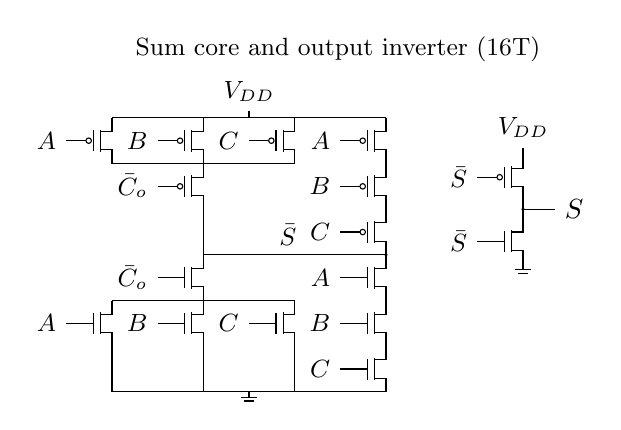
\begin{tikzpicture}[scale=.58]
\mos{0}{5.5}{A}{1}\mos{2}{5.5}{B}{1}\mos{4}{5.5}{C}{1}\mos{2}{4.5}{\bar C_o}{1}
\mos{6}{5.5}{A}{1}\mos{6}{4.5}{B}{1}\mos{6}{3.5}{C}{1}
\draw (.25,6)--(6.25,6);\rail{3.25}{6}{V_{DD}}\draw (.25,5)--(4.25,5);
\draw (2.25,4)--(2.25,3)--(6.25,3);\fill (6.25,3) circle (.04);\node[above,font=\small] at (4.1,3){$\bar S$};
\mos{2}{2.5}{\bar C_o}{0}\mos{0}{1.5}{A}{0}\mos{2}{1.5}{B}{0}\mos{4}{1.5}{C}{0}\draw (.25,2)--(4.25,2);
\mos{6}{2.5}{A}{0}\mos{6}{1.5}{B}{0}\mos{6}{.5}{C}{0}
\draw (.25,1)--(.25,0)--(6.25,0);\draw (2.25,1)--(2.25,0);\draw (4.25,1)--(4.25,0);\ground{3.25}{0}
\mos{9}{4.7}{\bar S}{1}\mos{9}{3.3}{\bar S}{0}\rail{9.25}{5.2}{V_{DD}}\ground{9.25}{2.8}\draw (9.25,3.8)--(9.25,4.2);\outputnode{9.25}{4}{S}
\node[font=\small] at (5.2,7.5){Sum core and output inverter (16T)};
\end{tikzpicture}\end{center}

\newpage\section*{Mirror sizing and exhaustive timing}
Core NMOS widths are 0.94 $\mu$m in two-device paths and 1.41 $\mu$m in three-device paths. Corresponding core PMOS widths are 3.76 and 5.64 $\mu$m (base PMOS strength factor 4). Both output NMOS widths are 0.47 $\mu$m. The separately tuned output PMOS widths are 2.117468 $\mu$m for carry and 2.949212 $\mu$m for sum. Every device length is 0.18 $\mu$m.

All 56 directed transitions between distinct 3-bit input words were run with simultaneous changing-input edges. All 112 settled-output checks pass. Output-changing transitions receive separate 50\%-to-50\% primary-input propagation-delay and 10--90\% slew measurements. The first changing input is the trigger; simultaneous edges share its 50\% time. The worst output delays from the final fine-step run are:
\begin{center}\begin{tabular}{lclrr}\toprule Output&Direction&Input transition&Delay (ps)&Slew (ps)\\\midrule
CO&LH&\texttt{000->110}&151.7633&47.5378\\
CO&HL&\texttt{110->100}&117.1854&40.6505\\
S&LH&\texttt{011->001}&246.9836&54.7344\\
S&HL&\texttt{010->110}&256.8529&44.0972\\
\bottomrule\end{tabular}\end{center}
\begin{center}\begin{tabular}{lrrr}\toprule Output&Worst rise (ps)&Worst fall (ps)&Difference (\%)\\\midrule
CO&47.9592&47.4564&1.048\\
S&56.5234&55.4221&1.948\\
\bottomrule\end{tabular}\end{center}
The matching metric compares the worst slews across cases; their input transitions need not be the same. Changing the maximum timestep from 1 ps to 0.2 ps changes any delay by at most 0.152698 ps. Delays use the first crossing in the intended direction after the input event; settled logic is checked independently. These measurements do not claim a general hazard-free settling bound for simultaneous multi-input transitions.

\newpage\section*{(b) Valid cascaded domino full adder}
Ordinary domino outputs reset low and rise monotonically during evaluation. Sum is not monotone in true A/B/C alone, so directly using the falling inverse of a domino carry as a sum input is unsafe. Instead generate two positive domino rails:
\[
C_o=AB+AC+BC,\qquad N_o=\bar A\bar B+\bar A\bar C+\bar B\bar C=\bar C_o.
\]
Input complements are generated by three static inverters and settle before evaluation. A third domino stage computes $S=N_o(A+B+C)+ABC$. Its positive $N_o$ input starts at 0 and may rise during evaluation, satisfying domino monotonicity. Both external outputs reset to 0 during precharge.

Each carry rail has a PMOS precharge, a clocked NMOS footer, a five-NMOS factored majority PDN, an output inverter, and a weak feedback PMOS keeper (10T). The sum stage uses a seven-NMOS PDN plus the same four supporting devices and keeper (12T). With 6 input-complement MOSFETs, total device count is $10+10+12+6=38$.

\textbf{Carry domino transistor diagram.} For the complement rail, repeat this same topology with A/B/C replaced by $\bar A/\bar B/\bar C$ and output $C_o$ replaced by $N_o$.
\begin{center}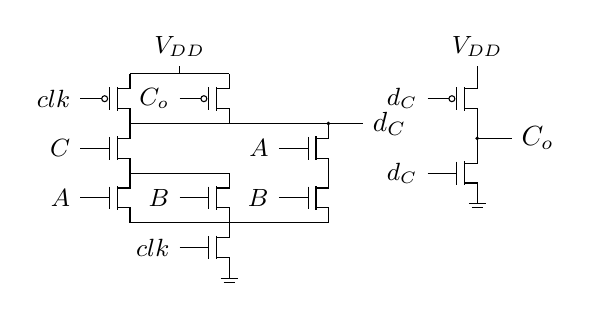
\begin{tikzpicture}[scale=.63]
\mos{0}{5}{clk}{1}\mos{2}{5}{C_o}{1}\draw (.25,5.5)--(2.25,5.5);\rail{1.25}{5.5}{V_{DD}}\draw (.25,4.5)--(4.25,4.5);\outputnode{4.25}{4.5}{d_C}
\mos{0}{4}{C}{0}\mos{0}{3}{A}{0}\mos{2}{3}{B}{0}\mos{4}{4}{A}{0}\mos{4}{3}{B}{0}\draw (.25,3.5)--(2.25,3.5);\draw (.25,2.5)--(4.25,2.5);
\mos{2}{2}{clk}{0}\ground{2.25}{1.5}
\mos{7}{5}{d_C}{1}\mos{7}{3.5}{d_C}{0}\rail{7.25}{5.5}{V_{DD}}\ground{7.25}{3}\draw (7.25,4)--(7.25,4.5);\outputnode{7.25}{4.2}{C_o}
\end{tikzpicture}\end{center}
All carry-PDN devices and its footer have width 1.41 $\mu$m. Precharge width is 1.88 $\mu$m. Keeper width is 0.47 $\mu$m with length 0.5 $\mu$m, so it is weak enough for evaluation to overcome it. The $N_o$ inverter uses NMOS 0.47 $\mu$m and PMOS 1.88 $\mu$m. External carry/sum inverter sizing is tuned separately below.

\newpage\section*{Domino sum transistor diagram and clock discipline}
\begin{center}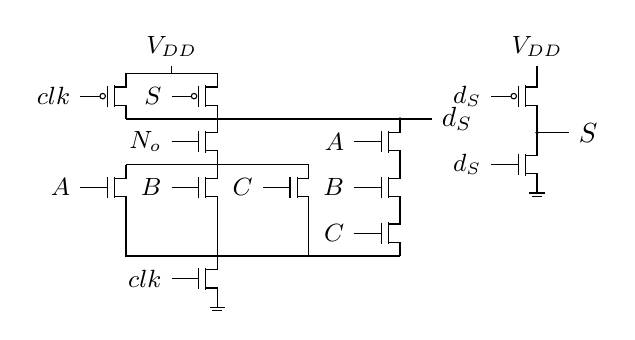
\begin{tikzpicture}[scale=.58]
\mos{0}{6}{clk}{1}\mos{2}{6}{S}{1}\draw (.25,6.5)--(2.25,6.5);\rail{1.25}{6.5}{V_{DD}}\draw (.25,5.5)--(6.25,5.5);\outputnode{6.25}{5.5}{d_S}
\mos{2}{5}{N_o}{0}\mos{0}{4}{A}{0}\mos{2}{4}{B}{0}\mos{4}{4}{C}{0}\draw (.25,4.5)--(4.25,4.5);
\mos{6}{5}{A}{0}\mos{6}{4}{B}{0}\mos{6}{3}{C}{0}
\draw (.25,3.5)--(.25,2.5)--(6.25,2.5);\draw (2.25,3.5)--(2.25,2.5);\draw (4.25,3.5)--(4.25,2.5);\mos{2}{2}{clk}{0}\ground{2.25}{1.5}
\mos{9}{6}{d_S}{1}\mos{9}{4.5}{d_S}{0}\rail{9.25}{6.5}{V_{DD}}\ground{9.25}{4}\draw (9.25,5)--(9.25,5.5);\outputnode{9.25}{5.2}{S}
\end{tikzpicture}\end{center}
The $N_o$ series device and the three parallel A/B/C NMOS devices are 1.41 $\mu$m wide. The ABC series branch and the common footer are 1.88 $\mu$m wide. Precharge is 1.88 $\mu$m wide and the keeper is 0.47/0.5 $\mu$m. Input inverters are $W_n=0.47$, $W_p=1.88$, $L=0.18\,\mu$m. All unlisted lengths are 0.18 $\mu$m. NMOS bodies use VSS and PMOS bodies use VDD.

Inputs and their complements are held stable for 2 ns before the clock rises and remain stable throughout evaluation. Clock rises over 20 ps at 2 ns, falls over 20 ps at 4 ns, and precharges until 5 ns. This explicit protocol avoids nonmonotone input changes and distinguishes an evaluate delay from reset delay. Weak keepers resist leakage and charge-sharing disturbance; every evaluated and reset word is checked electrically.

Both external output NMOS widths are 0.47 $\mu$m. The tuned output PMOS widths are 1.600841 $\mu$m for carry and 1.247602 $\mu$m for sum. Slew balance remains within 3\% in the fine-step simulation:
\begin{center}\begin{tabular}{lrrr}\toprule Output&Worst evaluate rise (ps)&Worst precharge fall (ps)&Difference (\%)\\\midrule
CO&46.1474&46.3049&0.340\\
S&50.2146&51.0225&1.583\\
\bottomrule\end{tabular}\end{center}

\newpage\section*{Domino truth table and measured timing}
All 8 input words pass for carry, sum, and the complementary carry rail; all three outputs reset below 0.2 V. The external binary outputs are:
\begin{center}\begin{tabular}{ccc|cc}\toprule A&B&C&Carry&Sum\\\midrule
0&0&0&0&0\\0&0&1&0&1\\0&1&0&0&1\\0&1&1&1&0\\1&0&0&0&1\\1&0&1&1&0\\1&1&0&1&0\\1&1&1&1&1\\\bottomrule\end{tabular}\end{center}
Domino evaluation delay is from the clock's rising 0.9 V crossing to the positive output's rising 0.9 V crossing, with data stable before the clock. Reset delay is from the falling clock crossing to the falling output. Low evaluate outputs never rise and do not receive a fictitious evaluation delay.
\begin{center}\begin{tabular}{lclrr}\toprule Output&Phase&Input word&Delay (ps)&Slew (ps)\\\midrule
CO&evaluate&\texttt{101}&91.1129&46.1474\\
CO&reset&\texttt{111}&110.7986&46.3049\\
S&evaluate&\texttt{100}&168.4105&50.2146\\
S&reset&\texttt{111}&114.7874&51.0225\\
\bottomrule\end{tabular}\end{center}
The timestep change modifies any domino timing measurement by at most 0.141547 ps. The sum's evaluate path may include the separate carry-complement stage. This latency is included in its clock-to-output delay, rather than measuring only the final inverter.

\newpage\section*{Actual schematic waveform examples}
The traces are embedded directly in this standalone source from measured voltage samples. The mirror example is its worst sum-fall transition, $010\to110$; the rising A input makes carry rise and sum fall after the internal carry-complement response. Time zero is the primary input 50\% crossing.
\begin{center}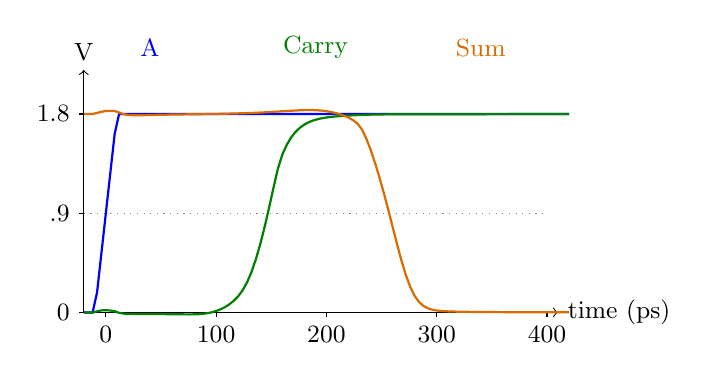
\begin{tikzpicture}[x=.014cm,y=1.4cm]
\draw[->] (0,0)--(430,0) node[right,font=\small]{time (ps)};\draw[->] (0,0)--(0,2.2) node[above,font=\small]{V};
\draw[dotted,gray] (0,.9)--(420,.9);
\foreach \x/\t in {20/0,120/100,220/200,320/300,420/400}{\draw (\x,0)--(\x,-.04) node[below,font=\small]{$\t$};}
\foreach \y in {0,.9,1.8}{\draw (0,\y)--(-4,\y) node[left,font=\small]{$\y$};}
\node[blue,font=\small] at (60,2.4){A};\node[green!50!black,font=\small] at (210,2.4){Carry};\node[orange!85!black,font=\small] at (360,2.4){Sum};
\draw[blue,thick] plot coordinates {(0.000,0.000000) (4.000,0.000000) (8.000,0.000000) (12.000,0.180000) (16.000,0.540000) (20.000,0.900000) (24.000,1.260000) (28.000,1.620000) (32.000,1.800000) (36.000,1.800000) (40.000,1.800000) (44.000,1.800000) (48.000,1.800000) (52.000,1.800000) (56.000,1.800000) (60.000,1.800000) (64.000,1.800000) (68.000,1.800000) (72.000,1.800000) (76.000,1.800000) (80.000,1.800000) (84.000,1.800000) (88.000,1.800000) (92.000,1.800000) (96.000,1.800000) (100.000,1.800000) (104.000,1.800000) (108.000,1.800000) (112.000,1.800000) (116.000,1.800000) (120.000,1.800000) (124.000,1.800000) (128.000,1.800000) (132.000,1.800000) (136.000,1.800000) (140.000,1.800000) (144.000,1.800000) (148.000,1.800000) (152.000,1.800000) (156.000,1.800000) (160.000,1.800000) (164.000,1.800000) (168.000,1.800000) (172.000,1.800000) (176.000,1.800000) (180.000,1.800000) (184.000,1.800000) (188.000,1.800000) (192.000,1.800000) (196.000,1.800000) (200.000,1.800000) (204.000,1.800000) (208.000,1.800000) (212.000,1.800000) (216.000,1.800000) (220.000,1.800000) (224.000,1.800000) (228.000,1.800000) (232.000,1.800000) (236.000,1.800000) (240.000,1.800000) (244.000,1.800000) (248.000,1.800000) (252.000,1.800000) (256.000,1.800000) (260.000,1.800000) (264.000,1.800000) (268.000,1.800000) (272.000,1.800000) (276.000,1.800000) (280.000,1.800000) (284.000,1.800000) (288.000,1.800000) (292.000,1.800000) (296.000,1.800000) (300.000,1.800000) (304.000,1.800000) (308.000,1.800000) (312.000,1.800000) (316.000,1.800000) (320.000,1.800000) (324.000,1.800000) (328.000,1.800000) (332.000,1.800000) (336.000,1.800000) (340.000,1.800000) (344.000,1.800000) (348.000,1.800000) (352.000,1.800000) (356.000,1.800000) (360.000,1.800000) (364.000,1.800000) (368.000,1.800000) (372.000,1.800000) (376.000,1.800000) (380.000,1.800000) (384.000,1.800000) (388.000,1.800000) (392.000,1.800000) (396.000,1.800000) (400.000,1.800000) (404.000,1.800000) (408.000,1.800000) (412.000,1.800000) (416.000,1.800000) (420.000,1.800000) (424.000,1.800000) (428.000,1.800000) (432.000,1.800000) (436.000,1.800000) (440.000,1.800000)};
\draw[green!50!black,thick] plot coordinates {(0.000,0.000000) (4.000,0.000000) (8.000,0.000000) (12.000,0.008991) (16.000,0.018242) (20.000,0.020088) (24.000,0.017303) (28.000,0.010128) (32.000,-0.003909) (36.000,-0.011053) (40.000,-0.013164) (44.000,-0.013762) (48.000,-0.013967) (52.000,-0.014118) (56.000,-0.014304) (60.000,-0.014541) (64.000,-0.014832) (68.000,-0.015185) (72.000,-0.015587) (76.000,-0.016033) (80.000,-0.016518) (84.000,-0.017032) (88.000,-0.017547) (92.000,-0.017986) (96.000,-0.018164) (100.000,-0.017715) (104.000,-0.016118) (108.000,-0.012826) (112.000,-0.007301) (116.000,0.000975) (120.000,0.012431) (124.000,0.027792) (128.000,0.047750) (132.000,0.073211) (136.000,0.105499) (140.000,0.146681) (144.000,0.200246) (148.000,0.271778) (152.000,0.365531) (156.000,0.481740) (160.000,0.619554) (164.000,0.776961) (168.000,0.950170) (172.000,1.132037) (176.000,1.303532) (180.000,1.430961) (184.000,1.520369) (188.000,1.587034) (192.000,1.637574) (196.000,1.675710) (200.000,1.704221) (204.000,1.725385) (208.000,1.741056) (212.000,1.752694) (216.000,1.761414) (220.000,1.768043) (224.000,1.773179) (228.000,1.777248) (232.000,1.780556) (236.000,1.783323) (240.000,1.785704) (244.000,1.787804) (248.000,1.789674) (252.000,1.791332) (256.000,1.792764) (260.000,1.793936) (264.000,1.794873) (268.000,1.795617) (272.000,1.796201) (276.000,1.796643) (280.000,1.796962) (284.000,1.797184) (288.000,1.797339) (292.000,1.797474) (296.000,1.797623) (300.000,1.797789) (304.000,1.797952) (308.000,1.798089) (312.000,1.798182) (316.000,1.798232) (320.000,1.798246) (324.000,1.798238) (328.000,1.798220) (332.000,1.798200) (336.000,1.798186) (340.000,1.798182) (344.000,1.798189) (348.000,1.798208) (352.000,1.798239) (356.000,1.798279) (360.000,1.798328) (364.000,1.798383) (368.000,1.798445) (372.000,1.798510) (376.000,1.798578) (380.000,1.798647) (384.000,1.798717) (388.000,1.798786) (392.000,1.798855) (396.000,1.798922) (400.000,1.798987) (404.000,1.799050) (408.000,1.799110) (412.000,1.799168) (416.000,1.799223) (420.000,1.799275) (424.000,1.799324) (428.000,1.799371) (432.000,1.799414) (436.000,1.799455) (440.000,1.799494)};
\draw[orange!85!black,thick] plot coordinates {(0.000,1.800000) (4.000,1.800000) (8.000,1.800000) (12.000,1.809373) (16.000,1.819884) (20.000,1.826394) (24.000,1.828170) (28.000,1.826866) (32.000,1.813112) (36.000,1.798422) (40.000,1.791916) (44.000,1.789252) (48.000,1.788514) (52.000,1.788744) (56.000,1.789449) (60.000,1.790359) (64.000,1.791327) (68.000,1.792273) (72.000,1.793157) (76.000,1.793961) (80.000,1.794680) (84.000,1.795316) (88.000,1.795878) (92.000,1.796378) (96.000,1.796841) (100.000,1.797301) (104.000,1.797793) (108.000,1.798336) (112.000,1.798944) (116.000,1.799628) (120.000,1.800399) (124.000,1.801260) (128.000,1.802190) (132.000,1.803182) (136.000,1.804228) (140.000,1.805333) (144.000,1.806510) (148.000,1.807784) (152.000,1.809197) (156.000,1.810802) (160.000,1.812660) (164.000,1.814801) (168.000,1.817145) (172.000,1.819582) (176.000,1.822041) (180.000,1.824474) (184.000,1.826844) (188.000,1.829149) (192.000,1.831358) (196.000,1.833348) (200.000,1.834880) (204.000,1.835644) (208.000,1.835291) (212.000,1.833515) (216.000,1.830117) (220.000,1.824977) (224.000,1.817997) (228.000,1.809048) (232.000,1.797958) (236.000,1.784358) (240.000,1.767163) (244.000,1.744890) (248.000,1.713877) (252.000,1.662746) (256.000,1.580732) (260.000,1.477298) (264.000,1.358221) (268.000,1.226315) (272.000,1.083856) (276.000,0.933016) (280.000,0.776471) (284.000,0.619205) (288.000,0.470479) (292.000,0.338896) (296.000,0.230833) (300.000,0.149550) (304.000,0.093672) (308.000,0.058134) (312.000,0.036760) (316.000,0.024296) (320.000,0.017072) (324.000,0.012810) (328.000,0.010192) (332.000,0.008486) (336.000,0.007293) (340.000,0.006399) (344.000,0.005688) (348.000,0.005097) (352.000,0.004591) (356.000,0.004149) (360.000,0.003757) (364.000,0.003408) (368.000,0.003095) (372.000,0.002813) (376.000,0.002559) (380.000,0.002330) (384.000,0.002122) (388.000,0.001934) (392.000,0.001764) (396.000,0.001609) (400.000,0.001469) (404.000,0.001341) (408.000,0.001226) (412.000,0.001120) (416.000,0.001024) (420.000,0.000937) (424.000,0.000858) (428.000,0.000785) (432.000,0.000719) (436.000,0.000659) (440.000,0.000604)};
\end{tikzpicture}\end{center}
For domino word $100$, the positive $N_o$ carry-complement rail rises first, then enables the sum PDN. Both reset during precharge. The full evaluation/reset phase trace below uses time since the clock ramp begins. Carry remains 0 for this word.
\begin{center}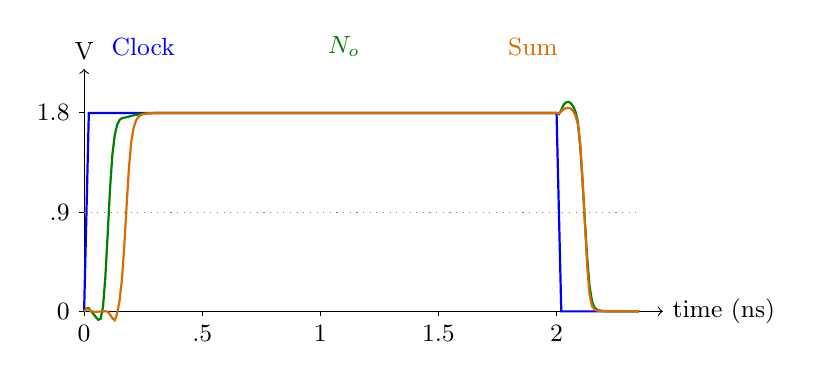
\begin{tikzpicture}[x=3cm,y=1.4cm]
\draw[->] (0,0)--(2.45,0) node[right,font=\small]{time (ns)};\draw[->] (0,0)--(0,2.2) node[above,font=\small]{V};
\draw[dotted,gray] (0,.9)--(2.35,.9);
\foreach \x in {0,.5,1,1.5,2}{\draw (\x,0)--(\x,-.04) node[below,font=\small]{$\x$};}
\foreach \y in {0,.9,1.8}{\draw (0,\y)--(-.02,\y) node[left,font=\small]{$\y$};}
\node[blue,font=\small] at (.25,2.4){Clock};\node[green!50!black,font=\small] at (1.1,2.4){$N_o$};\node[orange!85!black,font=\small] at (1.9,2.4){Sum};
\draw[blue,thick] plot coordinates {(0.0000,0.000000) (0.0100,0.900000) (0.0200,1.800000) (0.0300,1.800000) (0.0400,1.800000) (0.0500,1.800000) (0.0600,1.800000) (0.0700,1.800000) (0.0800,1.800000) (0.0900,1.800000) (0.1000,1.800000) (0.1100,1.800000) (0.1200,1.800000) (0.1300,1.800000) (0.1400,1.800000) (0.1500,1.800000) (0.1600,1.800000) (0.1700,1.800000) (0.1800,1.800000) (0.1900,1.800000) (0.2000,1.800000) (0.2100,1.800000) (0.2200,1.800000) (0.2300,1.800000) (0.2400,1.800000) (0.2500,1.800000) (0.2600,1.800000) (0.2700,1.800000) (0.2800,1.800000) (0.2900,1.800000) (0.3000,1.800000) (0.3100,1.800000) (0.3200,1.800000) (0.3300,1.800000) (0.3400,1.800000) (0.3500,1.800000) (0.3600,1.800000) (0.3700,1.800000) (0.3800,1.800000) (0.3900,1.800000) (0.4000,1.800000) (0.4100,1.800000) (0.4200,1.800000) (0.4300,1.800000) (0.4400,1.800000) (0.4500,1.800000) (0.4600,1.800000) (0.4700,1.800000) (0.4800,1.800000) (0.4900,1.800000) (0.5000,1.800000) (0.5100,1.800000) (0.5200,1.800000) (0.5300,1.800000) (0.5400,1.800000) (0.5500,1.800000) (0.5600,1.800000) (0.5700,1.800000) (0.5800,1.800000) (0.5900,1.800000) (0.6000,1.800000) (0.6100,1.800000) (0.6200,1.800000) (0.6300,1.800000) (0.6400,1.800000) (0.6500,1.800000) (0.6600,1.800000) (0.6700,1.800000) (0.6800,1.800000) (0.6900,1.800000) (0.7000,1.800000) (0.7100,1.800000) (0.7200,1.800000) (0.7300,1.800000) (0.7400,1.800000) (0.7500,1.800000) (0.7600,1.800000) (0.7700,1.800000) (0.7800,1.800000) (0.7900,1.800000) (0.8000,1.800000) (0.8100,1.800000) (0.8200,1.800000) (0.8300,1.800000) (0.8400,1.800000) (0.8500,1.800000) (0.8600,1.800000) (0.8700,1.800000) (0.8800,1.800000) (0.8900,1.800000) (0.9000,1.800000) (0.9100,1.800000) (0.9200,1.800000) (0.9300,1.800000) (0.9400,1.800000) (0.9500,1.800000) (0.9600,1.800000) (0.9700,1.800000) (0.9800,1.800000) (0.9900,1.800000) (1.0000,1.800000) (1.0100,1.800000) (1.0200,1.800000) (1.0300,1.800000) (1.0400,1.800000) (1.0500,1.800000) (1.0600,1.800000) (1.0700,1.800000) (1.0800,1.800000) (1.0900,1.800000) (1.1000,1.800000) (1.1100,1.800000) (1.1200,1.800000) (1.1300,1.800000) (1.1400,1.800000) (1.1500,1.800000) (1.1600,1.800000) (1.1700,1.800000) (1.1800,1.800000) (1.1900,1.800000) (1.2000,1.800000) (1.2100,1.800000) (1.2200,1.800000) (1.2300,1.800000) (1.2400,1.800000) (1.2500,1.800000) (1.2600,1.800000) (1.2700,1.800000) (1.2800,1.800000) (1.2900,1.800000) (1.3000,1.800000) (1.3100,1.800000) (1.3200,1.800000) (1.3300,1.800000) (1.3400,1.800000) (1.3500,1.800000) (1.3600,1.800000) (1.3700,1.800000) (1.3800,1.800000) (1.3900,1.800000) (1.4000,1.800000) (1.4100,1.800000) (1.4200,1.800000) (1.4300,1.800000) (1.4400,1.800000) (1.4500,1.800000) (1.4600,1.800000) (1.4700,1.800000) (1.4800,1.800000) (1.4900,1.800000) (1.5000,1.800000) (1.5100,1.800000) (1.5200,1.800000) (1.5300,1.800000) (1.5400,1.800000) (1.5500,1.800000) (1.5600,1.800000) (1.5700,1.800000) (1.5800,1.800000) (1.5900,1.800000) (1.6000,1.800000) (1.6100,1.800000) (1.6200,1.800000) (1.6300,1.800000) (1.6400,1.800000) (1.6500,1.800000) (1.6600,1.800000) (1.6700,1.800000) (1.6800,1.800000) (1.6900,1.800000) (1.7000,1.800000) (1.7100,1.800000) (1.7200,1.800000) (1.7300,1.800000) (1.7400,1.800000) (1.7500,1.800000) (1.7600,1.800000) (1.7700,1.800000) (1.7800,1.800000) (1.7900,1.800000) (1.8000,1.800000) (1.8100,1.800000) (1.8200,1.800000) (1.8300,1.800000) (1.8400,1.800000) (1.8500,1.800000) (1.8600,1.800000) (1.8700,1.800000) (1.8800,1.800000) (1.8900,1.800000) (1.9000,1.800000) (1.9100,1.800000) (1.9200,1.800000) (1.9300,1.800000) (1.9400,1.800000) (1.9500,1.800000) (1.9600,1.800000) (1.9700,1.800000) (1.9800,1.800000) (1.9900,1.800000) (2.0000,1.800000) (2.0100,0.900000) (2.0200,0.000000) (2.0300,0.000000) (2.0400,0.000000) (2.0500,0.000000) (2.0600,0.000000) (2.0700,0.000000) (2.0800,0.000000) (2.0900,0.000000) (2.1000,0.000000) (2.1100,0.000000) (2.1200,0.000000) (2.1300,0.000000) (2.1400,0.000000) (2.1500,0.000000) (2.1600,0.000000) (2.1700,0.000000) (2.1800,0.000000) (2.1900,0.000000) (2.2000,0.000000) (2.2100,0.000000) (2.2200,0.000000) (2.2300,0.000000) (2.2400,0.000000) (2.2500,0.000000) (2.2600,0.000000) (2.2700,0.000000) (2.2800,0.000000) (2.2900,0.000000) (2.3000,0.000000) (2.3100,0.000000) (2.3200,0.000000) (2.3300,0.000000) (2.3400,0.000000) (2.3500,0.000000)};
\draw[green!50!black,thick] plot coordinates {(0.0000,0.000000) (0.0100,0.027134) (0.0200,0.027468) (0.0300,-0.001406) (0.0400,-0.024320) (0.0500,-0.052602) (0.0600,-0.076514) (0.0700,-0.067130) (0.0800,0.040297) (0.0900,0.313932) (0.1000,0.706720) (0.1100,1.121360) (0.1200,1.429352) (0.1300,1.602280) (0.1400,1.693031) (0.1500,1.736496) (0.1600,1.751967) (0.1700,1.756774) (0.1800,1.761047) (0.1900,1.766928) (0.2000,1.773258) (0.2100,1.778504) (0.2200,1.783009) (0.2300,1.786897) (0.2400,1.790148) (0.2500,1.792753) (0.2600,1.794762) (0.2700,1.796264) (0.2800,1.797361) (0.2900,1.798150) (0.3000,1.798710) (0.3100,1.799103) (0.3200,1.799379) (0.3300,1.799570) (0.3400,1.799703) (0.3500,1.799795) (0.3600,1.799859) (0.3700,1.799903) (0.3800,1.799933) (0.3900,1.799954) (0.4000,1.799968) (0.4100,1.799978) (0.4200,1.799985) (0.4300,1.799990) (0.4400,1.799993) (0.4500,1.799995) (0.4600,1.799997) (0.4700,1.799998) (0.4800,1.799998) (0.4900,1.799999) (0.5000,1.799999) (0.5100,1.799999) (0.5200,1.800000) (0.5300,1.800000) (0.5400,1.800000) (0.5500,1.800000) (0.5600,1.800000) (0.5700,1.800000) (0.5800,1.800000) (0.5900,1.800000) (0.6000,1.800000) (0.6100,1.800000) (0.6200,1.800000) (0.6300,1.800000) (0.6400,1.800000) (0.6500,1.800000) (0.6600,1.800000) (0.6700,1.800000) (0.6800,1.800000) (0.6900,1.800000) (0.7000,1.800000) (0.7100,1.800000) (0.7200,1.800000) (0.7300,1.800000) (0.7400,1.800000) (0.7500,1.800000) (0.7600,1.800000) (0.7700,1.800000) (0.7800,1.800000) (0.7900,1.800000) (0.8000,1.800000) (0.8100,1.800000) (0.8200,1.800000) (0.8300,1.800000) (0.8400,1.800000) (0.8500,1.800000) (0.8600,1.800000) (0.8700,1.800000) (0.8800,1.800000) (0.8900,1.800000) (0.9000,1.800000) (0.9100,1.800000) (0.9200,1.800000) (0.9300,1.800000) (0.9400,1.800000) (0.9500,1.800000) (0.9600,1.800000) (0.9700,1.800000) (0.9800,1.800000) (0.9900,1.800000) (1.0000,1.800000) (1.0100,1.800000) (1.0200,1.800000) (1.0300,1.800000) (1.0400,1.800000) (1.0500,1.800000) (1.0600,1.800000) (1.0700,1.800000) (1.0800,1.800000) (1.0900,1.800000) (1.1000,1.800000) (1.1100,1.800000) (1.1200,1.800000) (1.1300,1.800000) (1.1400,1.800000) (1.1500,1.800000) (1.1600,1.800000) (1.1700,1.800000) (1.1800,1.800000) (1.1900,1.800000) (1.2000,1.800000) (1.2100,1.800000) (1.2200,1.800000) (1.2300,1.800000) (1.2400,1.800000) (1.2500,1.800000) (1.2600,1.800000) (1.2700,1.800000) (1.2800,1.800000) (1.2900,1.800000) (1.3000,1.800000) (1.3100,1.800000) (1.3200,1.800000) (1.3300,1.800000) (1.3400,1.800000) (1.3500,1.800000) (1.3600,1.800000) (1.3700,1.800000) (1.3800,1.800000) (1.3900,1.800000) (1.4000,1.800000) (1.4100,1.800000) (1.4200,1.800000) (1.4300,1.800000) (1.4400,1.800000) (1.4500,1.800000) (1.4600,1.800000) (1.4700,1.800000) (1.4800,1.800000) (1.4900,1.800000) (1.5000,1.800000) (1.5100,1.800000) (1.5200,1.800000) (1.5300,1.800000) (1.5400,1.800000) (1.5500,1.800000) (1.5600,1.800000) (1.5700,1.800000) (1.5800,1.800000) (1.5900,1.800000) (1.6000,1.800000) (1.6100,1.800000) (1.6200,1.800000) (1.6300,1.800000) (1.6400,1.800000) (1.6500,1.800000) (1.6600,1.800000) (1.6700,1.800000) (1.6800,1.800000) (1.6900,1.800000) (1.7000,1.800000) (1.7100,1.800000) (1.7200,1.800000) (1.7300,1.800000) (1.7400,1.800000) (1.7500,1.800000) (1.7600,1.800000) (1.7700,1.800000) (1.7800,1.800000) (1.7900,1.800000) (1.8000,1.800000) (1.8100,1.800000) (1.8200,1.800000) (1.8300,1.800000) (1.8400,1.800000) (1.8500,1.800000) (1.8600,1.800000) (1.8700,1.800000) (1.8800,1.800000) (1.8900,1.800000) (1.9000,1.800000) (1.9100,1.800000) (1.9200,1.800000) (1.9300,1.800000) (1.9400,1.800000) (1.9500,1.800000) (1.9600,1.800000) (1.9700,1.800000) (1.9800,1.800000) (1.9900,1.800000) (2.0000,1.800000) (2.0100,1.788356) (2.0200,1.826998) (2.0300,1.875513) (2.0400,1.894791) (2.0500,1.900560) (2.0600,1.889628) (2.0700,1.861136) (2.0800,1.812967) (2.0900,1.723362) (2.1000,1.496249) (2.1100,1.180818) (2.1200,0.820997) (2.1300,0.479193) (2.1400,0.226803) (2.1500,0.091548) (2.1600,0.036887) (2.1700,0.016883) (2.1800,0.008966) (2.1900,0.005304) (2.2000,0.003358) (2.2100,0.002229) (2.2200,0.001539) (2.2300,0.001102) (2.2400,0.000818) (2.2500,0.000626) (2.2600,0.000494) (2.2700,0.000400) (2.2800,0.000331) (2.2900,0.000278) (2.3000,0.000238) (2.3100,0.000205) (2.3200,0.000179) (2.3300,0.000158) (2.3400,0.000140) (2.3500,0.000125)};
\draw[orange!85!black,thick] plot coordinates {(0.0000,0.000000) (0.0100,0.019936) (0.0200,0.020115) (0.0300,0.000051) (0.0400,-0.002622) (0.0500,-0.002825) (0.0600,-0.002649) (0.0700,-0.002077) (0.0800,-0.000935) (0.0900,0.000887) (0.1000,-0.003117) (0.1100,-0.030457) (0.1200,-0.062935) (0.1300,-0.080367) (0.1400,-0.018882) (0.1500,0.096331) (0.1600,0.286964) (0.1700,0.588935) (0.1800,0.961073) (0.1900,1.307482) (0.2000,1.542189) (0.2100,1.668452) (0.2200,1.732768) (0.2300,1.764622) (0.2400,1.780491) (0.2500,1.788661) (0.2600,1.793082) (0.2700,1.795613) (0.2800,1.797139) (0.2900,1.798099) (0.3000,1.798721) (0.3100,1.799133) (0.3200,1.799410) (0.3300,1.799597) (0.3400,1.799724) (0.3500,1.799811) (0.3600,1.799870) (0.3700,1.799911) (0.3800,1.799939) (0.3900,1.799958) (0.4000,1.799971) (0.4100,1.799980) (0.4200,1.799986) (0.4300,1.799991) (0.4400,1.799994) (0.4500,1.799996) (0.4600,1.799997) (0.4700,1.799998) (0.4800,1.799999) (0.4900,1.799999) (0.5000,1.799999) (0.5100,1.799999) (0.5200,1.800000) (0.5300,1.800000) (0.5400,1.800000) (0.5500,1.800000) (0.5600,1.800000) (0.5700,1.800000) (0.5800,1.800000) (0.5900,1.800000) (0.6000,1.800000) (0.6100,1.800000) (0.6200,1.800000) (0.6300,1.800000) (0.6400,1.800000) (0.6500,1.800000) (0.6600,1.800000) (0.6700,1.800000) (0.6800,1.800000) (0.6900,1.800000) (0.7000,1.800000) (0.7100,1.800000) (0.7200,1.800000) (0.7300,1.800000) (0.7400,1.800000) (0.7500,1.800000) (0.7600,1.800000) (0.7700,1.800000) (0.7800,1.800000) (0.7900,1.800000) (0.8000,1.800000) (0.8100,1.800000) (0.8200,1.800000) (0.8300,1.800000) (0.8400,1.800000) (0.8500,1.800000) (0.8600,1.800000) (0.8700,1.800000) (0.8800,1.800000) (0.8900,1.800000) (0.9000,1.800000) (0.9100,1.800000) (0.9200,1.800000) (0.9300,1.800000) (0.9400,1.800000) (0.9500,1.800000) (0.9600,1.800000) (0.9700,1.800000) (0.9800,1.800000) (0.9900,1.800000) (1.0000,1.800000) (1.0100,1.800000) (1.0200,1.800000) (1.0300,1.800000) (1.0400,1.800000) (1.0500,1.800000) (1.0600,1.800000) (1.0700,1.800000) (1.0800,1.800000) (1.0900,1.800000) (1.1000,1.800000) (1.1100,1.800000) (1.1200,1.800000) (1.1300,1.800000) (1.1400,1.800000) (1.1500,1.800000) (1.1600,1.800000) (1.1700,1.800000) (1.1800,1.800000) (1.1900,1.800000) (1.2000,1.800000) (1.2100,1.800000) (1.2200,1.800000) (1.2300,1.800000) (1.2400,1.800000) (1.2500,1.800000) (1.2600,1.800000) (1.2700,1.800000) (1.2800,1.800000) (1.2900,1.800000) (1.3000,1.800000) (1.3100,1.800000) (1.3200,1.800000) (1.3300,1.800000) (1.3400,1.800000) (1.3500,1.800000) (1.3600,1.800000) (1.3700,1.800000) (1.3800,1.800000) (1.3900,1.800000) (1.4000,1.800000) (1.4100,1.800000) (1.4200,1.800000) (1.4300,1.800000) (1.4400,1.800000) (1.4500,1.800000) (1.4600,1.800000) (1.4700,1.800000) (1.4800,1.800000) (1.4900,1.800000) (1.5000,1.800000) (1.5100,1.800000) (1.5200,1.800000) (1.5300,1.800000) (1.5400,1.800000) (1.5500,1.800000) (1.5600,1.800000) (1.5700,1.800000) (1.5800,1.800000) (1.5900,1.800000) (1.6000,1.800000) (1.6100,1.800000) (1.6200,1.800000) (1.6300,1.800000) (1.6400,1.800000) (1.6500,1.800000) (1.6600,1.800000) (1.6700,1.800000) (1.6800,1.800000) (1.6900,1.800000) (1.7000,1.800000) (1.7100,1.800000) (1.7200,1.800000) (1.7300,1.800000) (1.7400,1.800000) (1.7500,1.800000) (1.7600,1.800000) (1.7700,1.800000) (1.7800,1.800000) (1.7900,1.800000) (1.8000,1.800000) (1.8100,1.800000) (1.8200,1.800000) (1.8300,1.800000) (1.8400,1.800000) (1.8500,1.800000) (1.8600,1.800000) (1.8700,1.800000) (1.8800,1.800000) (1.8900,1.800000) (1.9000,1.800000) (1.9100,1.800000) (1.9200,1.800000) (1.9300,1.800000) (1.9400,1.800000) (1.9500,1.800000) (1.9600,1.800000) (1.9700,1.800000) (1.9800,1.800000) (1.9900,1.800000) (2.0000,1.800000) (2.0100,1.795225) (2.0200,1.814539) (2.0300,1.834761) (2.0400,1.842208) (2.0500,1.845760) (2.0600,1.840905) (2.0700,1.818854) (2.0800,1.775218) (2.0900,1.700754) (2.1000,1.534409) (2.1100,1.195739) (2.1200,0.791898) (2.1300,0.401406) (2.1400,0.149941) (2.1500,0.048227) (2.1600,0.017918) (2.1700,0.008367) (2.1800,0.004466) (2.1900,0.002513) (2.2000,0.001447) (2.2100,0.000847) (2.2200,0.000505) (2.2300,0.000308) (2.2400,0.000194) (2.2500,0.000127) (2.2600,0.000086) (2.2700,0.000062) (2.2800,0.000046) (2.2900,0.000036) (2.3000,0.000029) (2.3100,0.000024) (2.3200,0.000020) (2.3300,0.000017) (2.3400,0.000015) (2.3500,0.000013)};
\end{tikzpicture}\end{center}
All worst-case waveform samples are included in \path{mirror_waveforms.csv} and \path{domino_waveforms.csv}, at 2 ps sampled spacing. Fine solver timing measurements use 0.2 ps maximum internal steps. These figures show the expected evaluation discipline and pipeline response; they are not replacements for the complete measured tables.
\newpage\section*{Source comparison and reproducibility}
The supplied \texttt{black.txt}, 4-1 code JPG, and archived \path{4.sp} match the instructor's 28T mirror topology. That topology is retained, while fixed historical widths are replaced by measured slew balancing. The historical delay directives trigger from internal complemented nodes, so they describe only output-inverter delay; the new static results use primary inputs and all 56 transitions.

The 4-2 JPG and \path{4D.sp} combine an n-type dynamic carry with a p-type dynamic sum using complementary clocks. That is a mixed n/p dynamic construction, not a conventional cascaded n-type domino implementation. The new 38T circuit uses proper precharge/footer/keeper stages and a positive complement-carry rail to meet the requested domino style. Historical incomplete input/clock coverage is replaced by all 8 evaluate words and reset checks. No legacy waveform value is relabeled as new evidence.

\begin{lstlisting}
python reproduce.py --model D:/cic018.l --raw-dir <scratch>
\end{lstlisting}
This regenerates netlists, performs and records the sizing search, verifies all cases, and runs fine-step checks. The directly runnable final decks are \path{mirror_testbench.sp} and \path{domino_testbench.sp}; netlists are \path{mirror.sp} and \path{domino.sp}. The local process library is not distributed. \path{sizing_search.csv} records every tuning step and \path{verification.json} records dimensions, counts, conventions, and hashes normalized to UTF-8 LF.

\end{document}
